\documentclass[1000pt]{article}
\pagenumbering{arabic}
\usepackage{mathptmx,amsmath}
\usepackage{pdfslide2}%,pause}
\usepackage{graphicx}
\usepackage{epstopdf}
\usepackage[T1]{fontenc} %need for portuguese caracters
\graphicspath{{./figures/}}
\usepackage{float}
\usepackage{tabularx}
\usepackage{braket}
\usepackage{multicol}
\usepackage{xcolor,colortbl}

\definecolor{itblue}{rgb}{0.0,0.0,0.5}
\definecolor{itred}{rgb}{0.82,0.18,0.24}

\definecolor{tab}{RGB}{0,82,136}
\definecolor{tab2}{RGB}{173,193,222}


\definecolor{title}{RGB}{68,85,95}
\definecolor{author}{RGB}{120,144,159}
\definecolor{author2}{RGB}{180,204,219}


\newcommand{\half}{\textstyle \frac{1}{2}}%
\newcommand{\fig}[2]{\colorbox{white}{\includegraphics[scale=#2]{#1}}}%
%\newcommand{\fig}[2]{\includegraphics[scale=#2]{#1}}%
\newcommand{\pd}[2]{\frac{\partial #1}{\partial #2}}%
\newcommand{\cb}[1]{{\color{itblue} #1}}%
\renewcommand{\labelitemi}{\textcolor{itred}{\normalsize $\bullet$}}
\renewcommand{\labelitemii}{\textcolor{green}{$\star$}}
\newcommand{\ave}[1]{\langle #1 \rangle}%
\newcommand{\mysection}[1]{\section*{\color{black}\sffamily #1}}%

\newcommand{\cref}[1]{{\fontsize{17pt}{0cm}\selectfont\color{black} #1}}%
\renewcommand*\footnoterule{}
\newcommand\blfootnote[1]{%
  \begingroup
  \renewcommand\thefootnote{}\footnote{#1}%
  \addtocounter{footnote}{-1}%
  \endgroup
}

\pagestyle{title}

\begin{document}

%------------TITLE SLIDE -------
\begin{titlepage}  \overlay{it_0.png}

\color{itblue} \sffamily \noindent \normalsize
\hspace*{4cm} Quantum Technologies, 2018/19\\
\hspace*{4cm} Physics Department, University of Aveiro\\
\\
\\
\hspace*{6.5cm}\begin{minipage}{15in}
\vspace*{2cm}
\begin{flushleft}
 \color{title} \sffamily \noindent \Huge
\textbf{Coherent One Way (COW) QKD Protocol}
\end{flushleft}
\end{minipage}
\vspace*{2cm}\\
\\
\hspace*{6.5cm}
%\begin{minipage}{7.5cm}
\color{author}
\Large João António$^1$, Daniel Pereira$^{2,3}$, Armando N. Pinto$^{2,3}$\\
%\end{minipage}\
\\
\vspace*{2cm}\\
\hspace*{6.5cm}
\begin{minipage}{12cm}
\color{title}
\large Physics Department$^1$,\\
Department of Electronics, Telecommunications and Informatics$^2$,\\
University of Aveiro, Aveiro, Portugal\\
Instituto de Telecomunica\c{c}\~{o}es,$^3$, Aveiro, Portugal
\end{minipage}\


\end{titlepage}


\mysection{\Huge\textbf{ Quantum Key Distribution}} \Large \vspace*{1cm}
\overlay{it_1.png}
\begin{itemize}
\item Quantum Key Distribution (QKD) is a secure way of create and share a unique random key between two spatially distant parties;
\item Discrete vs Continuous QKD;
\item Codification on polarization or time bins.
\end{itemize}
  \begin{figure}[hbt]
    	\centering
    	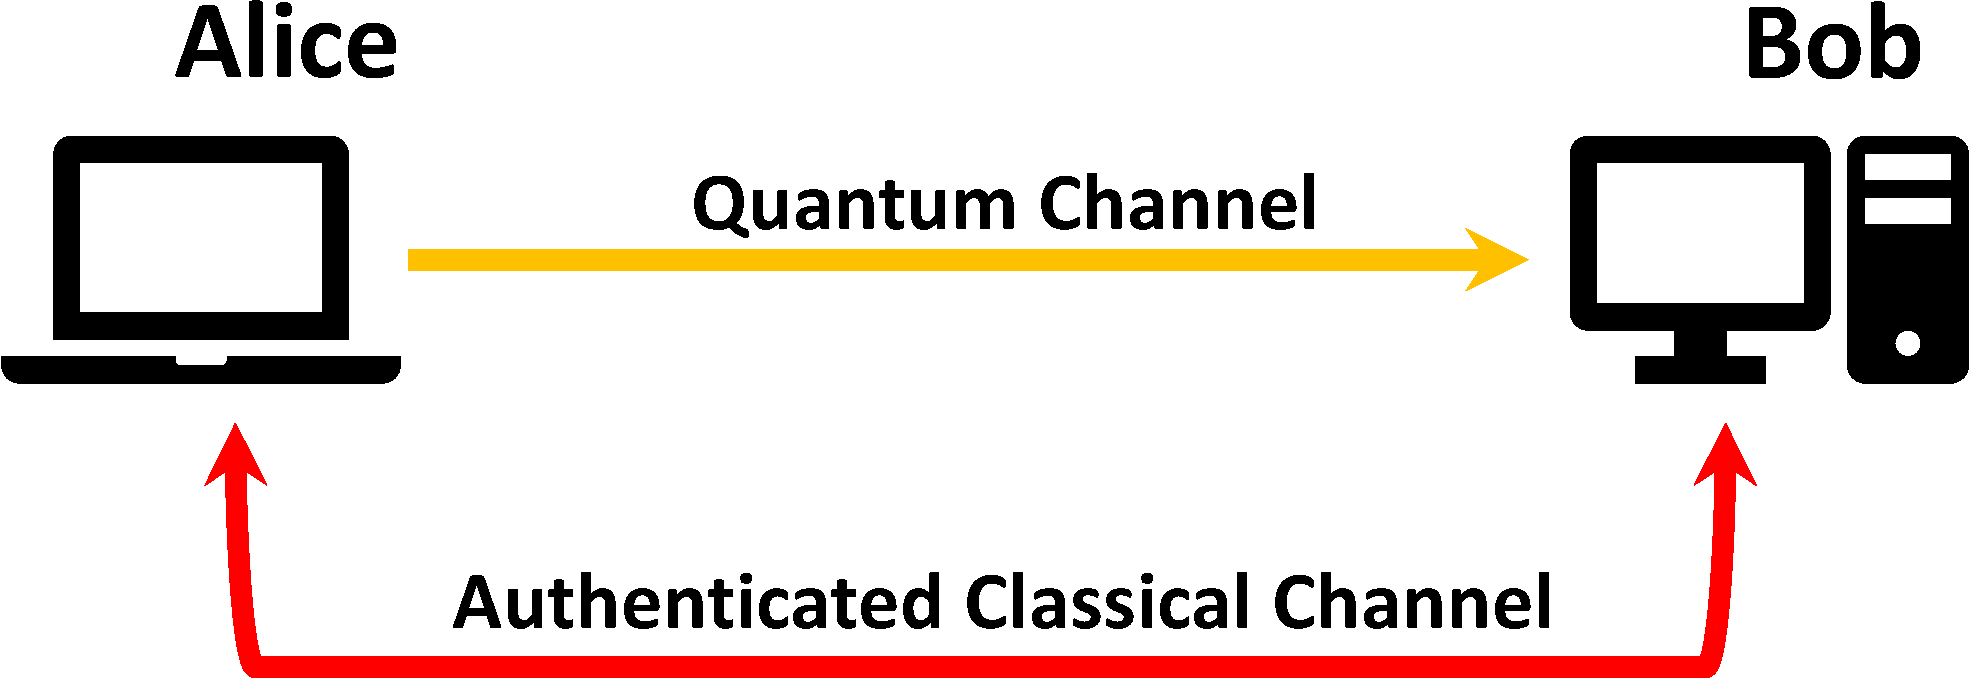
\includegraphics[width=0.6\textwidth]{./figures/Full.pdf}
    \end{figure}
       
\blfootnote{
\hspace*{12cm}
\begin{minipage}{26cm}
\cref{
Ouellette, Jennifer. "Quantum key distribution." Industrial Physicist 10.6 (2004): 22-25.
}
\end{minipage}

}
%%%%%%%%%%%%%%%%%%%%%%%%%%%%%%
%------------ SLIDE 1 -------%
%%%%%%%%%%%%%%%%%%%%%%%%%%%%%%
\mysection{\Huge\textbf{Time Bin QKD}} \Large \vspace*{1cm}
\begin{itemize}

\item The Coherent One Way (COW) protocol was elaborated by Nicolas Gisin et al in 2004. 

\item Uses discrete variables and time bin encoding.

\item It is has a very simple setup.
\end{itemize}
    \begin{figure}[hbt]
    	\centering
    	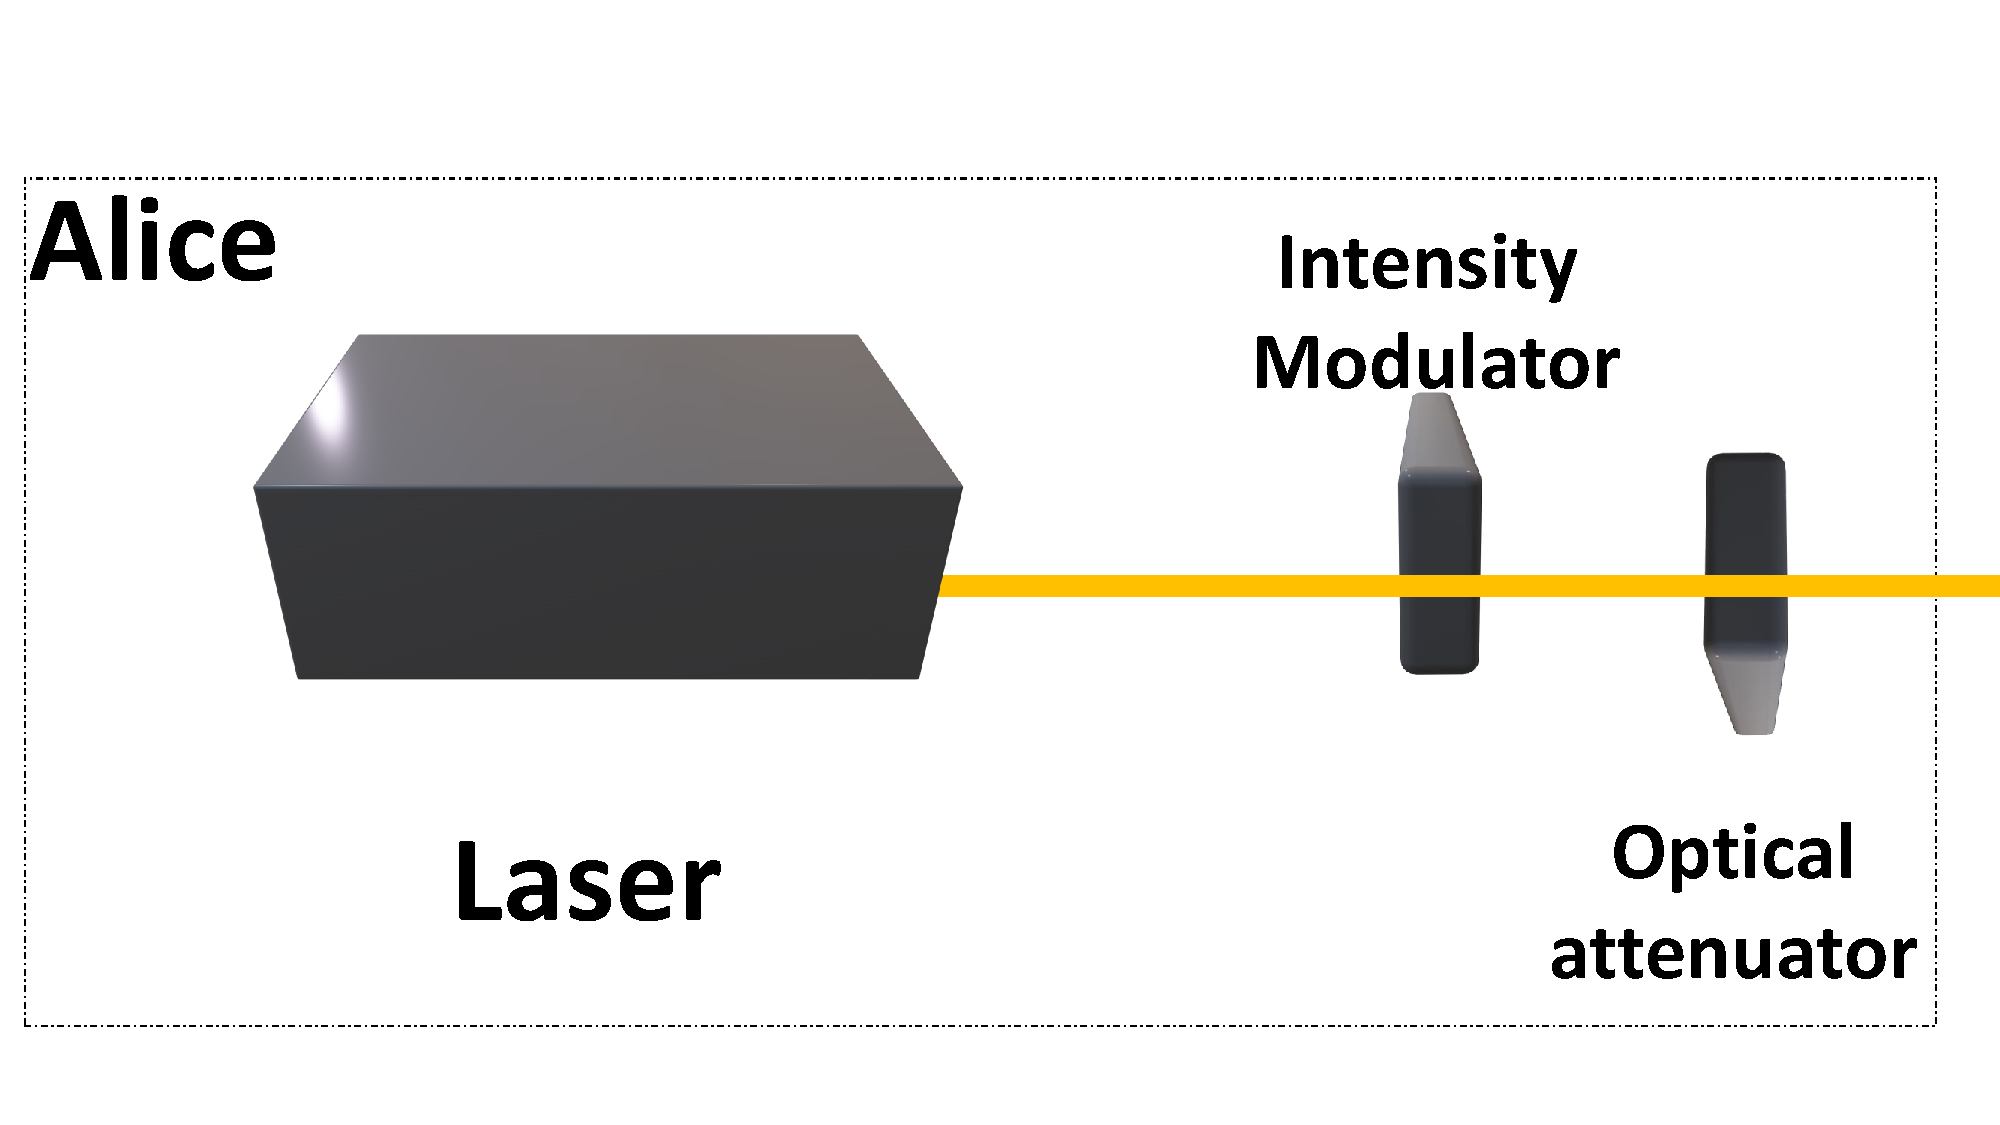
\includegraphics[width=0.6\textwidth]{./figures/A.pdf}
        	\label{bob}
    \end{figure}
    
\blfootnote{
\hspace*{12cm}
\begin{minipage}{26cm}
\cref{
Gisin, Nicolas, et al. "Towards practical and fast quantum cryptography." arXiv preprint quant-ph/0411022 (2004)
}
\end{minipage}
}

%%%%%%%%%%%%%%%%%%%%%%%%%%%%%%
%------------ SLIDE x -------%
%%%%%%%%%%%%%%%%%%%%%%%%%%%%%%
\mysection{\Huge\textbf{Alice}} \Large \vspace*{1cm}

\begin{description}

\item[Step 1] Alice creates a random key using: 
 
\end{description}

$$|0\rangle = |\alpha\rangle |\emptyset\rangle =\ \ Logical\ 0\ $$
  $$|1\rangle = |\emptyset\rangle |\alpha\rangle =\ \ Logical\ 1\ $$
$$|d\rangle = |\alpha\rangle |\alpha\rangle = Decoy State$$

Where $|\emptyset\rangle$ is the vacuum state and $|\alpha\rangle$ is a coherent state of light. The average number of photons by impulse is modulated by a Poisson distribution with $\lambda=0.1$.

    \begin{figure}[hbt]
    	\centering
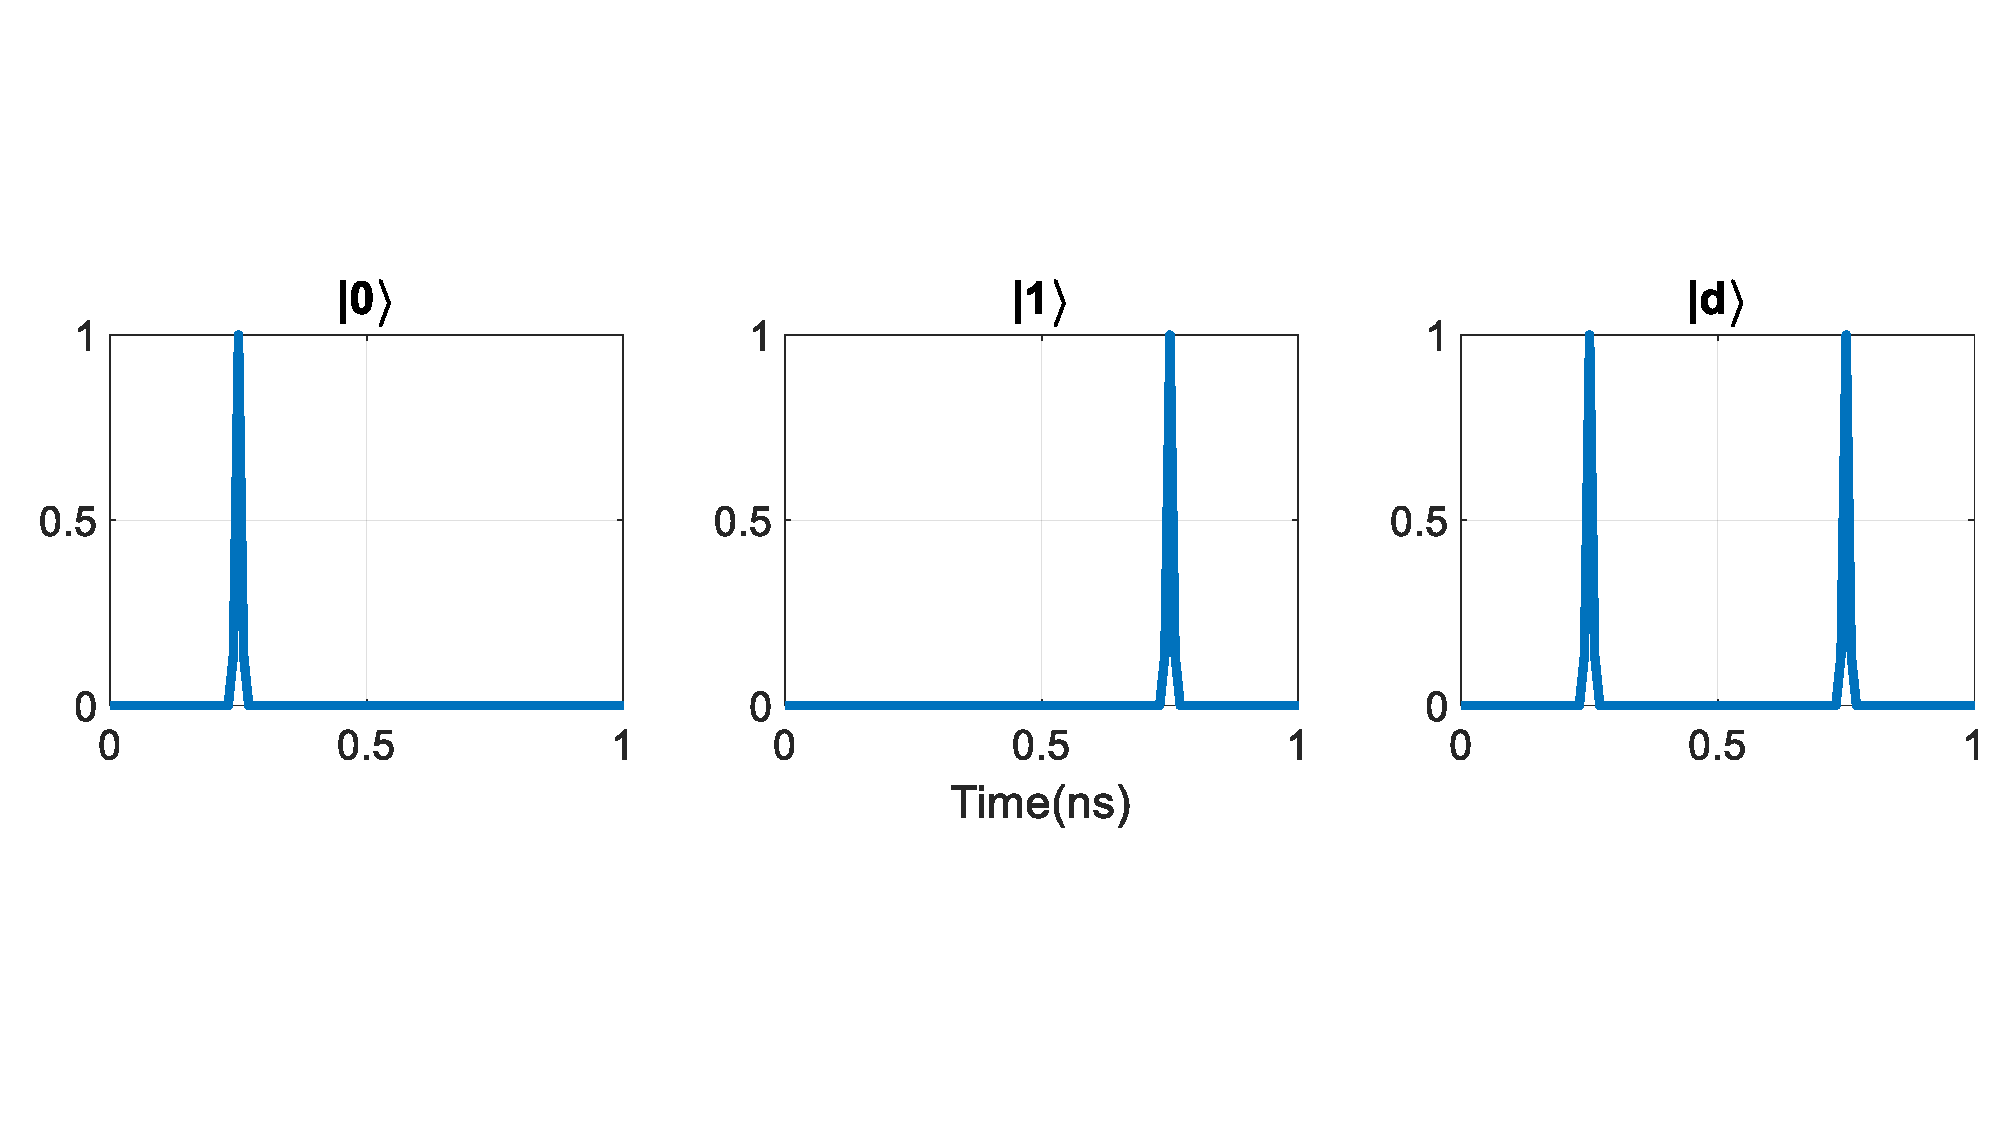
\includegraphics[width=0.6\textwidth]{./figures/S1.pdf}
        	\label{bob}
    \end{figure}




%--------------------------------------------------------------------------------------------------
%------------ SLIDE -------------------------------------------------------------------------------

\mysection{\Huge\textbf{Bob}} \Large \vspace*{1cm}

\begin{description}
  \item[Step 2] A fraction $t_B$ of the photons go into the photon counter $D_B$, where the bits are discriminated by the time of arrival and are used to create the key.
\end{description}  

Half of the other photons are delayed by 0.5 $t_{bit}$ interacting with the half of non-delayed bits.
    \begin{figure}[hbt]
    	\centering
    	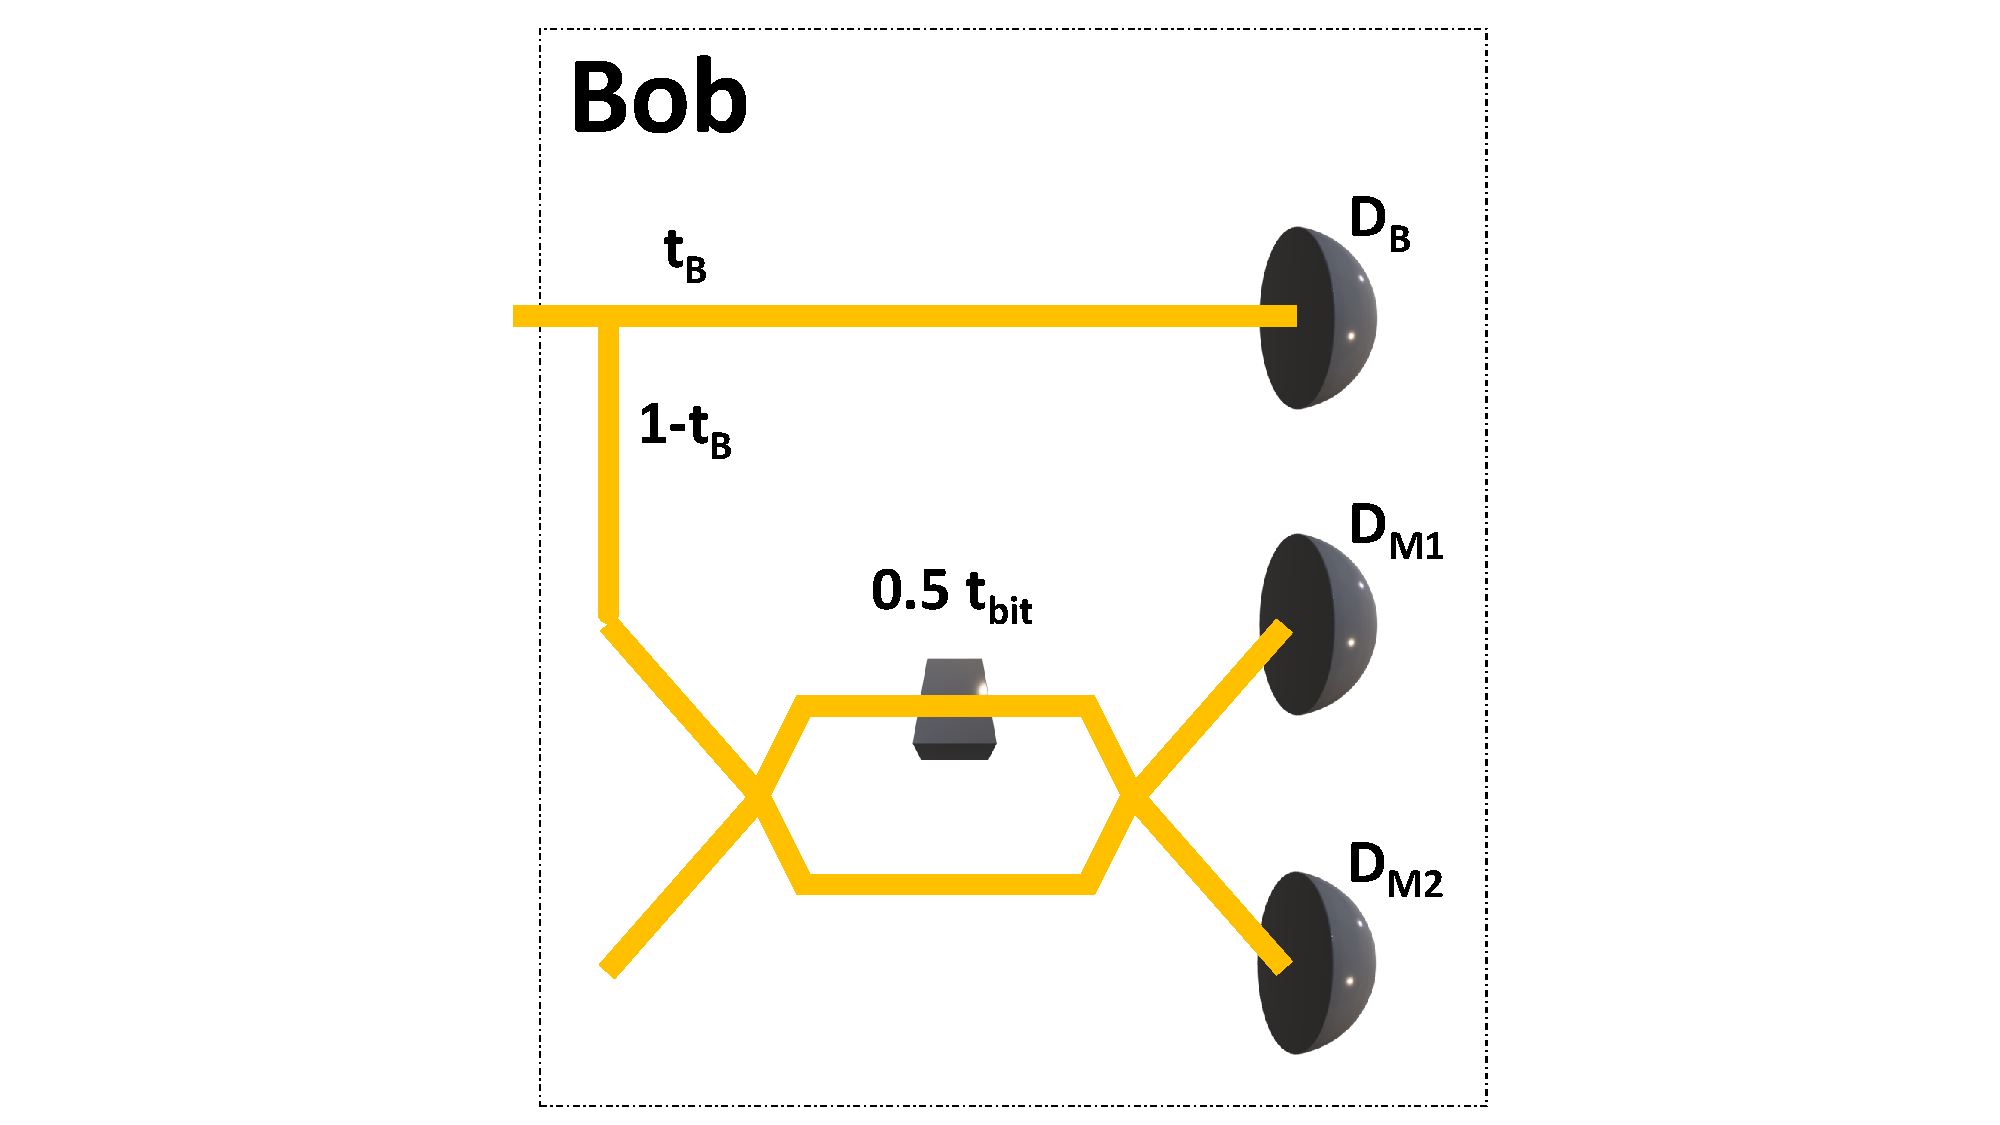
\includegraphics[width=0.6\textwidth]{./figures/B.pdf}
    \end{figure}
%--------------------------------------------------------------------------------------------------
%------------ SLIDE -------------------------------------------------------------------------------
\mysection{\Huge\textbf{Monitoring line clicks}} \Large \vspace*{1cm}

Therefore $D_{M2}$ (constructive photon counter) should only click when, the two pulses go to the monitoring line and the first impulse is delayed:
\vspace*{0.5cm}
    \begin{figure}[hbt]
    	\centering
    	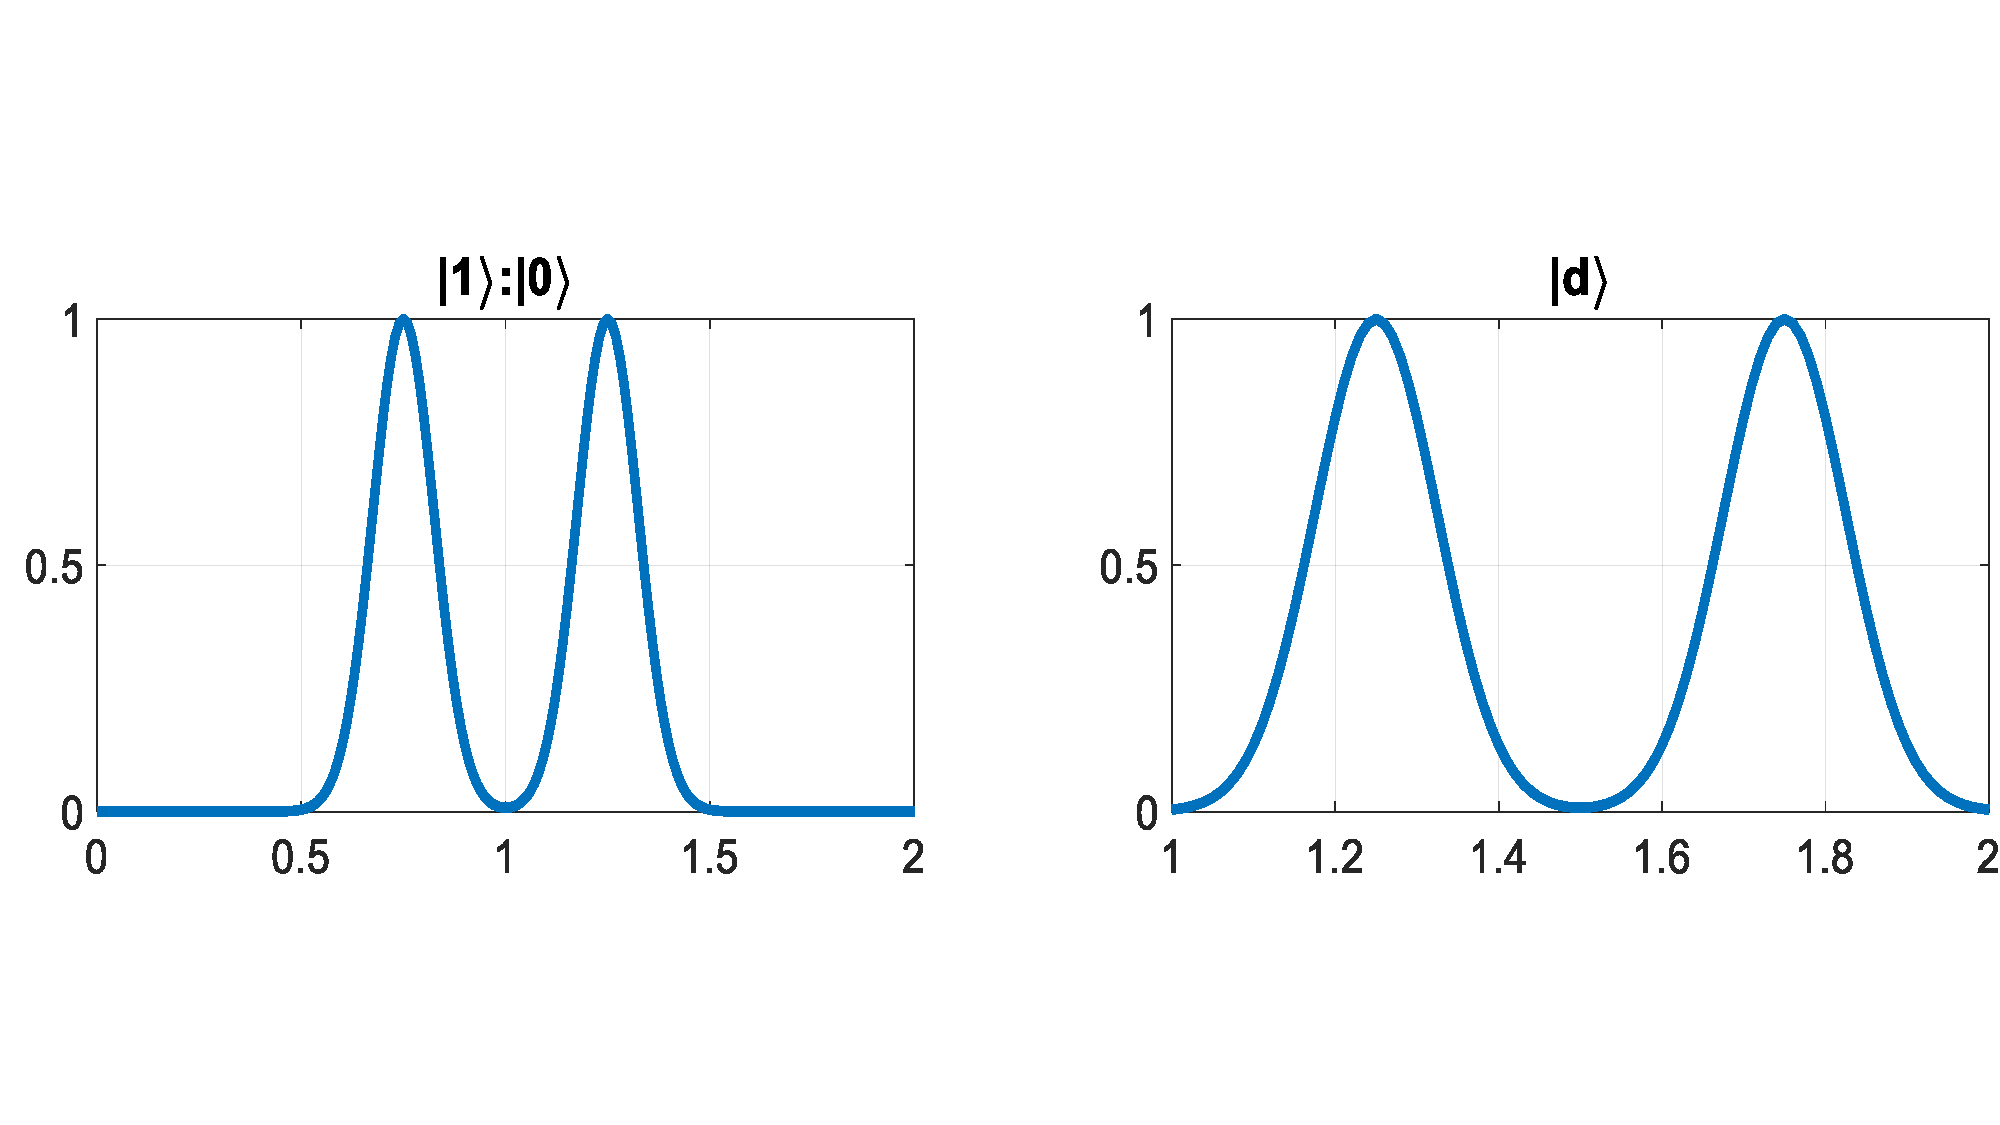
\includegraphics[width=1\textwidth]{./figures/S2.pdf}
    \end{figure}
%--------------------------------------------------------------------------------------------------
%------------ SLIDE -------------------------------------------------------------------------------

\mysection{\Huge\textbf{Monitoring line example}} \Large \vspace*{1cm}

Supposing that all impulses have multiple photons, and all go to the monitoring line.

  \begin{figure}[hbt]
    	\centering
    	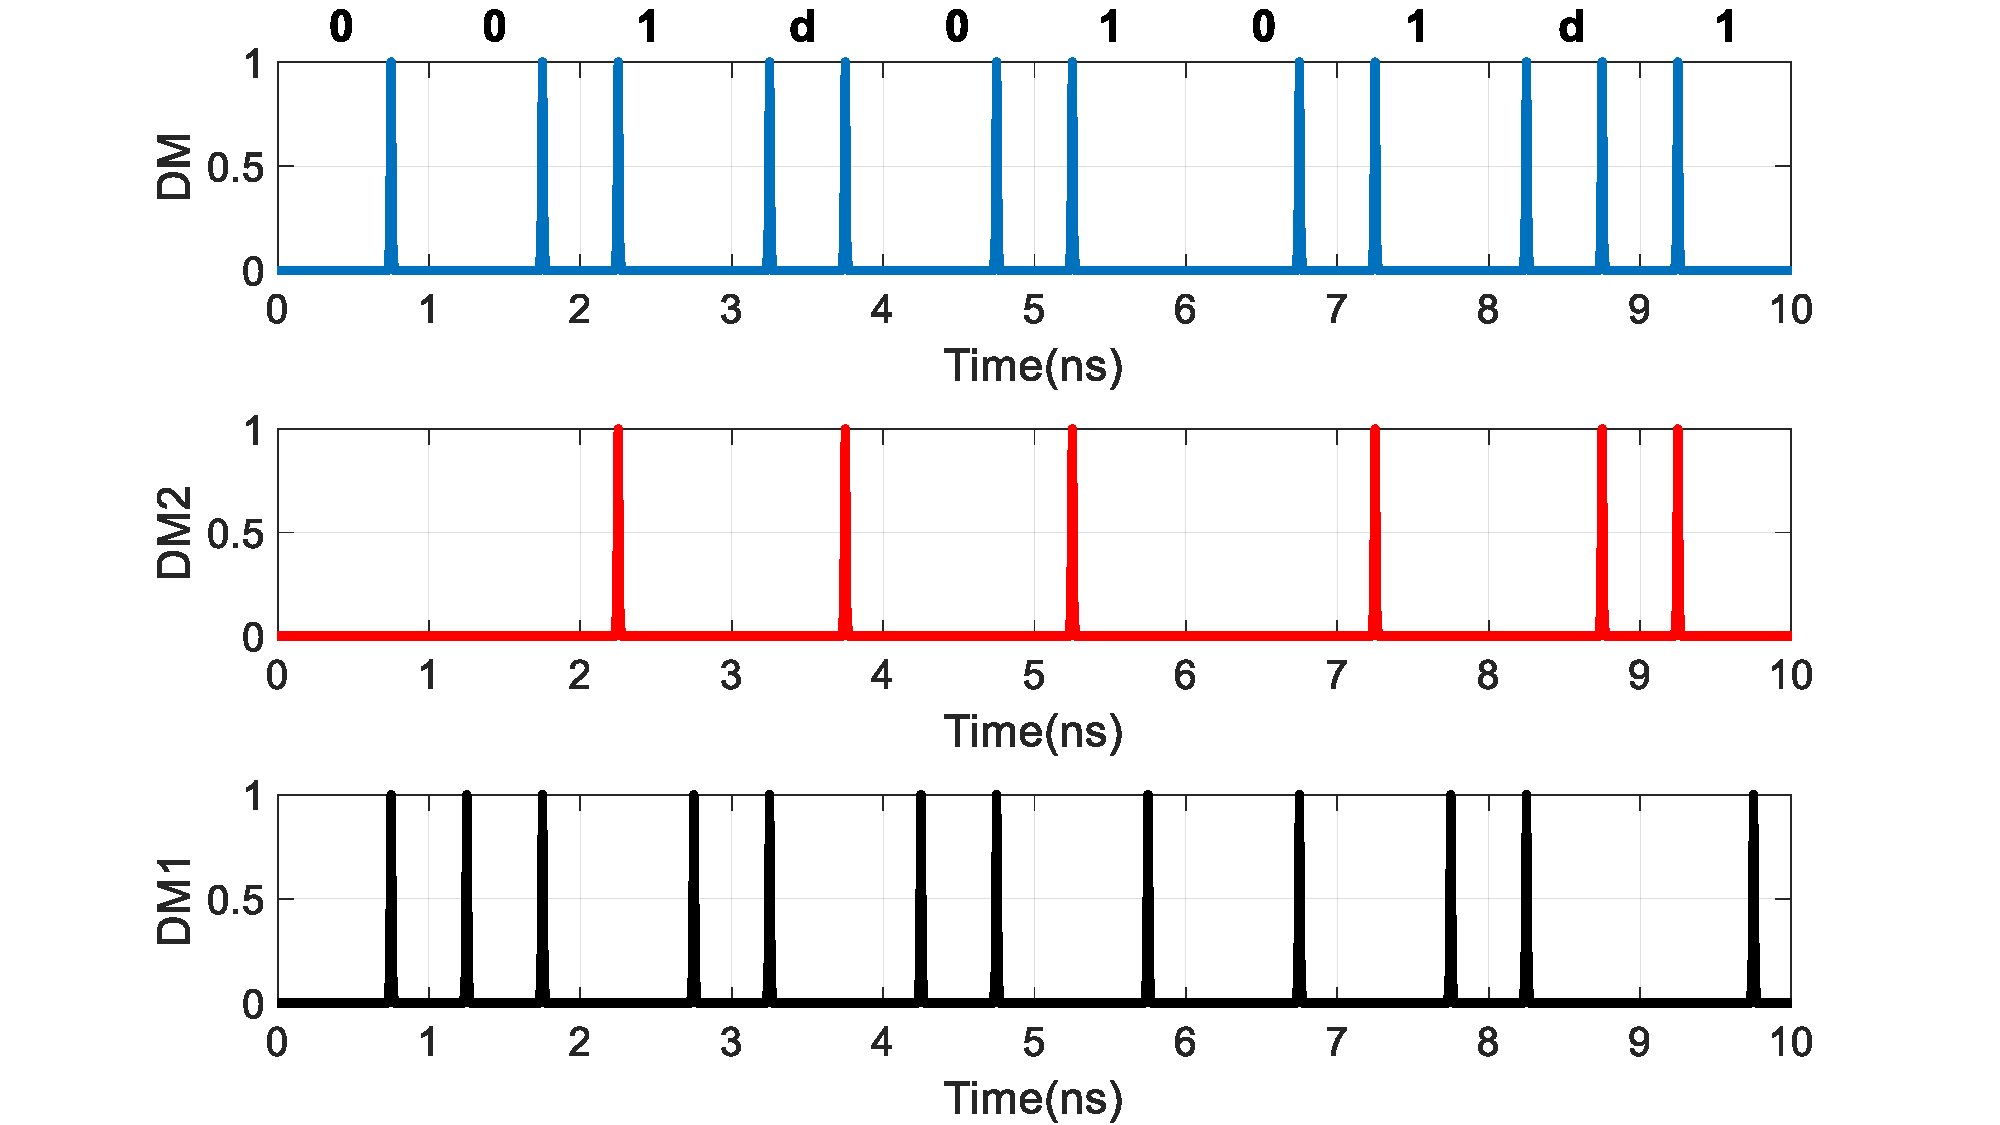
\includegraphics[width=0.75\textwidth]{./figures/DM3.pdf}
    \end{figure}

%--------------------------------------------------------------------------------------------------
%------------ SLIDE -------------------------------------------------------------------------------

\mysection{\Huge\textbf{Testing Visibility and Errors}} \Large \vspace*{1cm}

\begin{description}

\item [Step 3] Alice tell the decoy times. Bob checks if the \textbf{$D_{M2}$} has fired during those times.

\item [Step 4] Bob reveals the other times that he had a detection in \textbf{$D_{M2}$}, Alice verifies if they belong to a $|1\rangle:|0\rangle$.

\item [Step 5] Bob reveals the times that $D_B$ fired, and they use those as key.

\item [Step 6] QBER, check the number of the detections for every detector.

\item [Step 7] Run error correction and privacy amplification.
\end{description}
\begin{figure}[hbt]
    	\centering
    	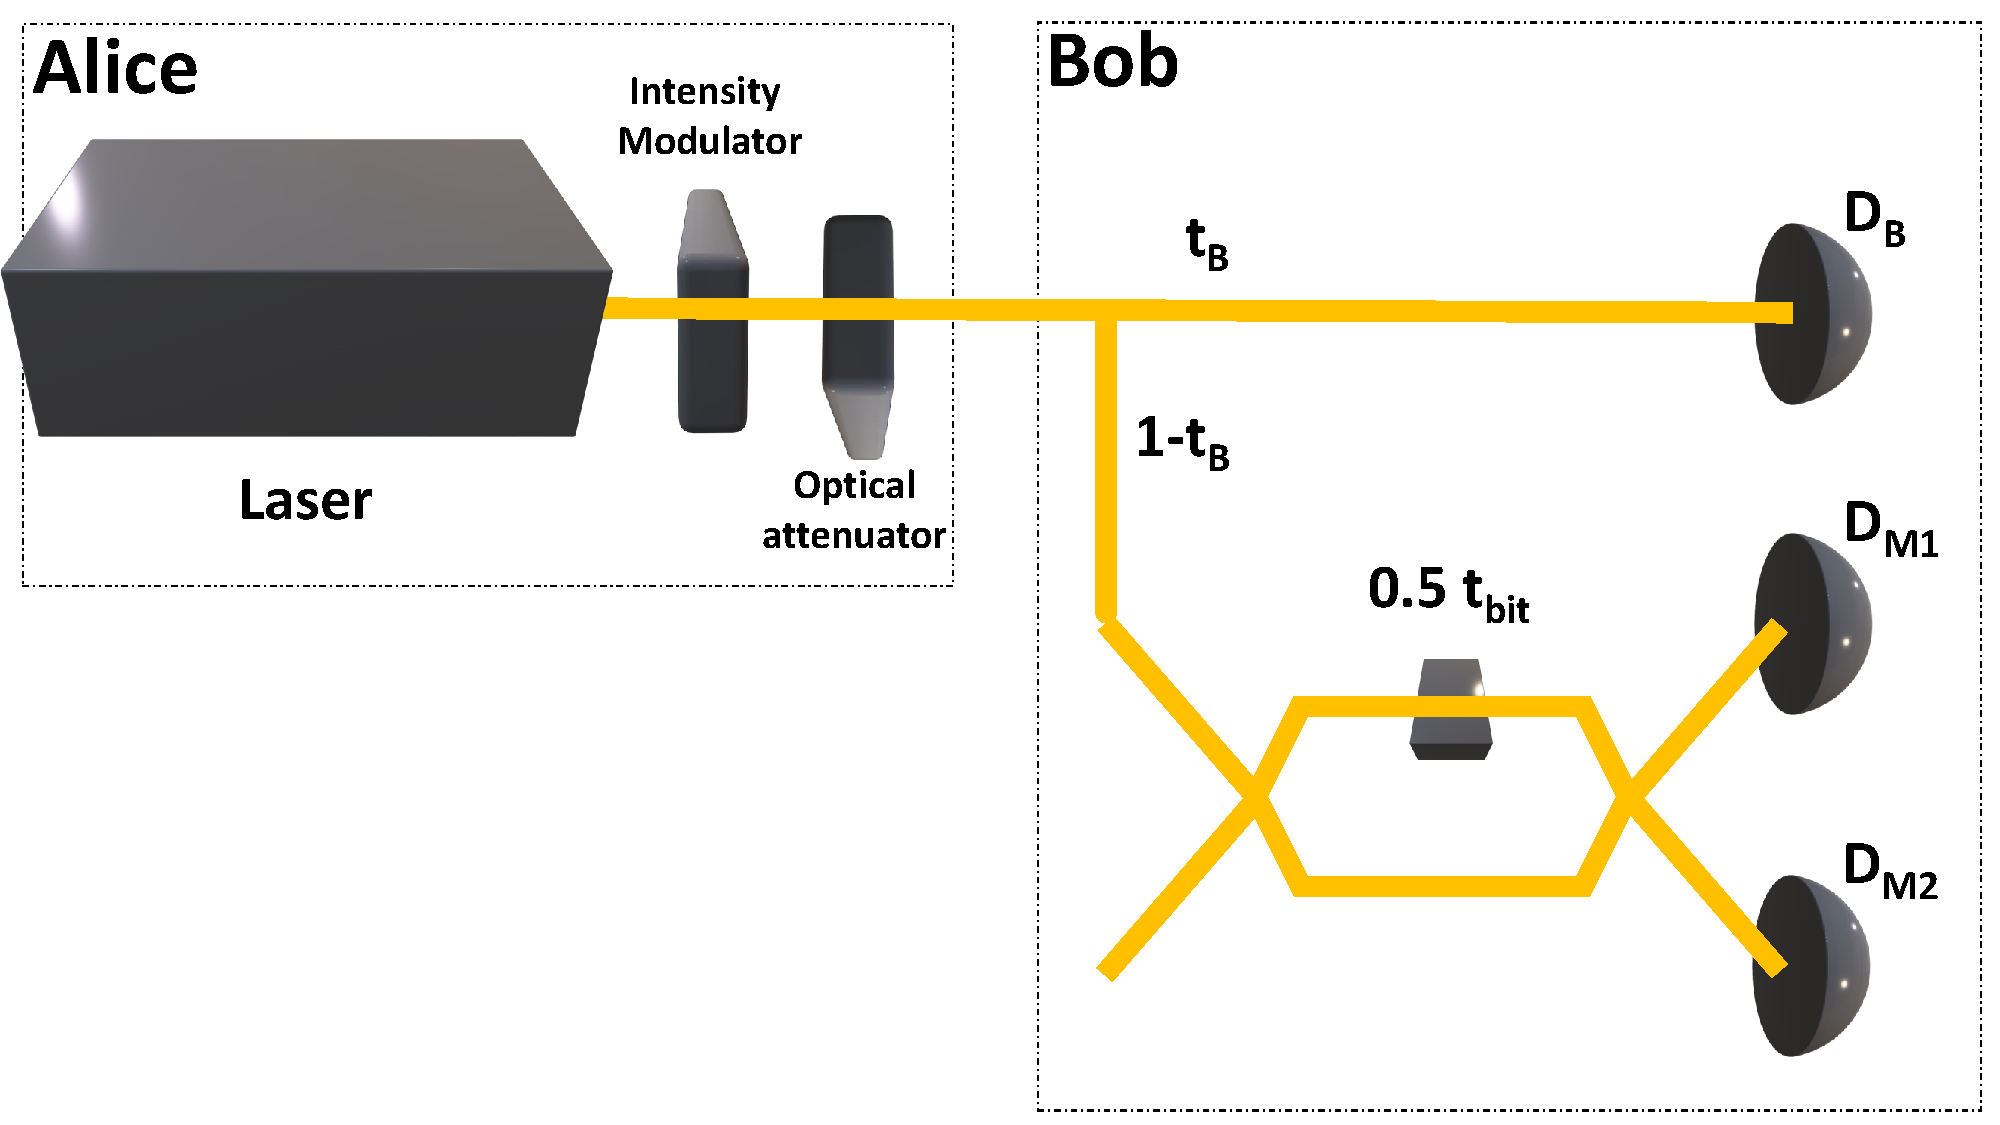
\includegraphics[width=0.45\textwidth]{./figures/Full2.pdf}
    \end{figure}

%--------------------------------------------------------------------------------------------------
%------------ SLIDE -------------------------------------------------------------------------------
\mysection{\Huge\textbf{Intercept-Resend Attack}} \Large \vspace*{1cm}

We want to see how robust is the protocol to a \textbf{Intercept-Resend Attack}. On this attack Eve captures all the information, measures and then resend it to Bob.

\begin{figure}[hbt]
    	\centering
    	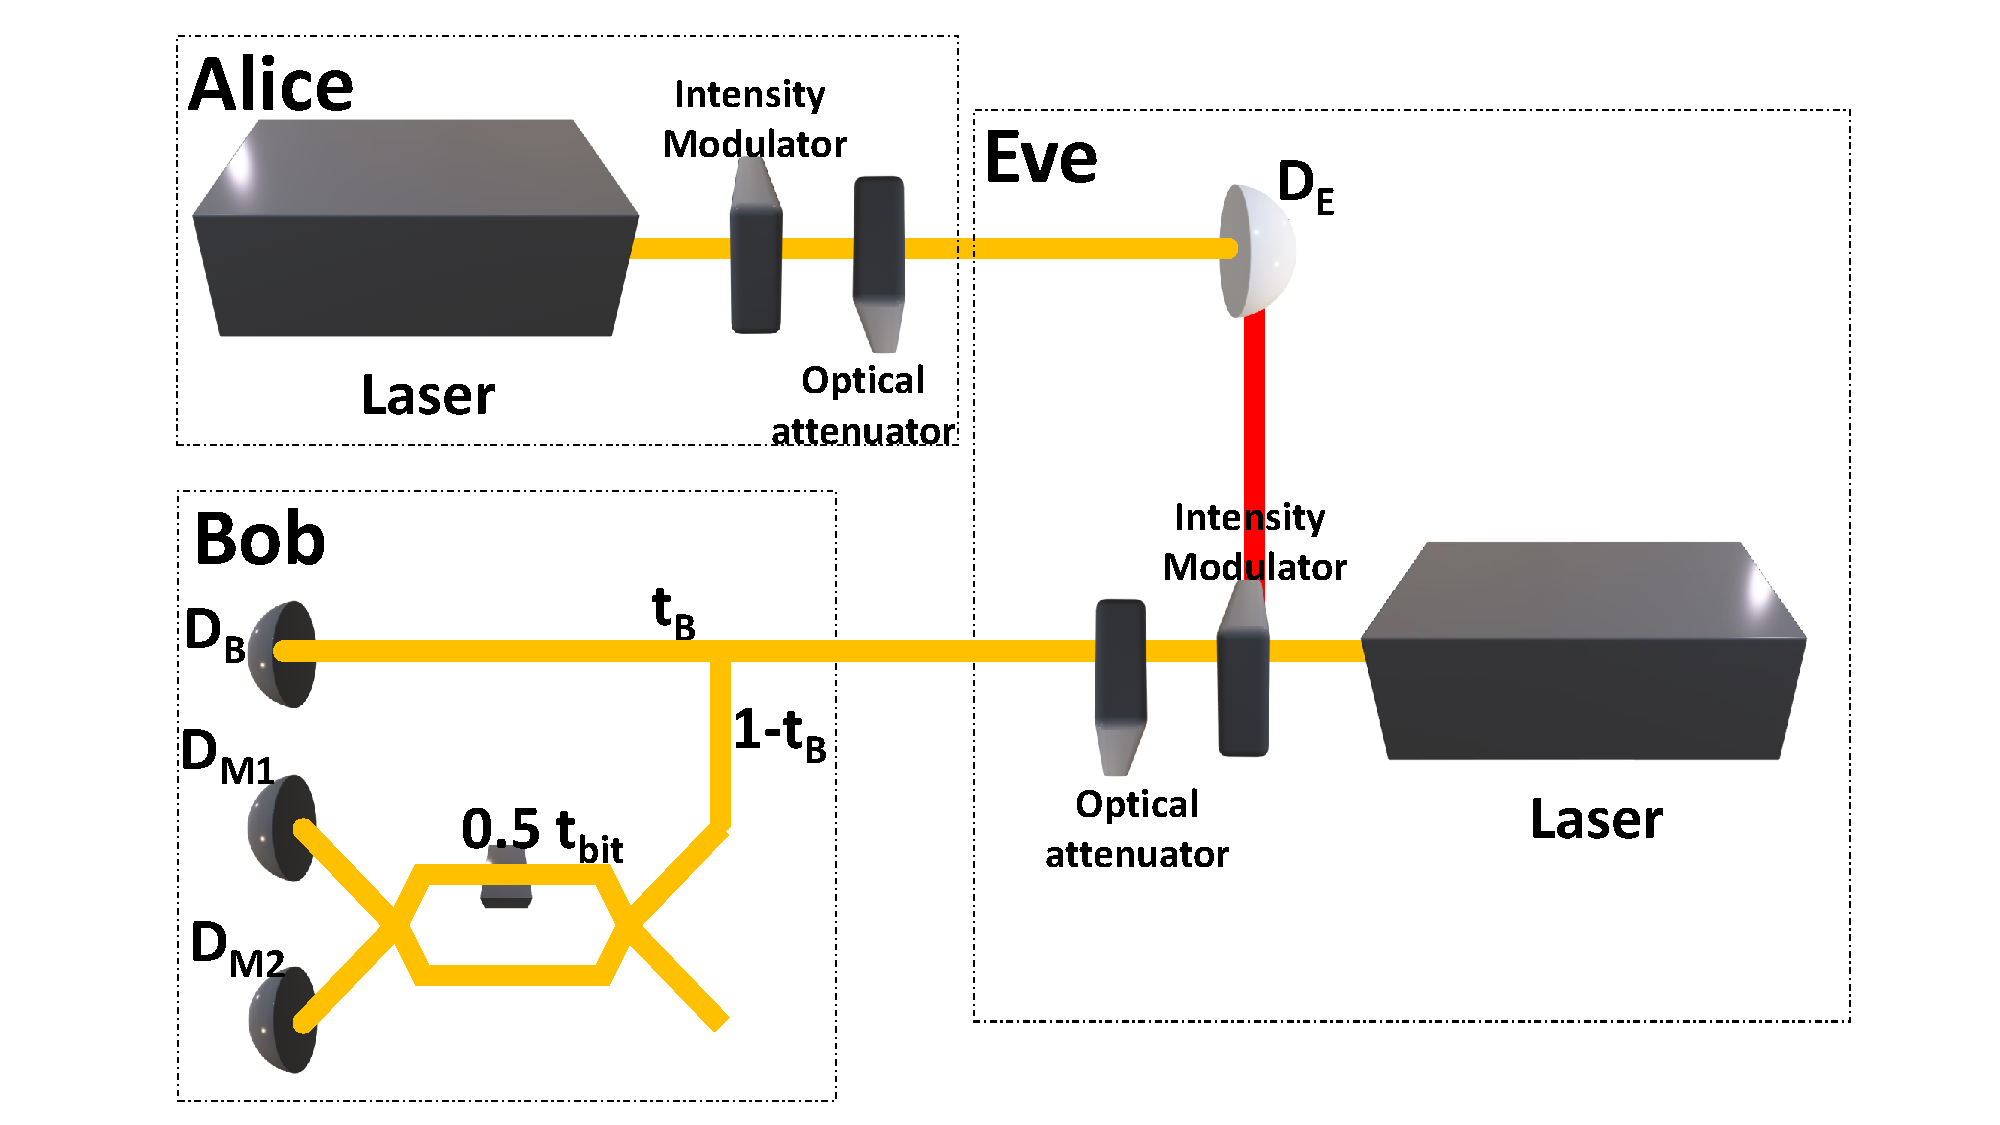
\includegraphics[width=0.7\textwidth]{./figures/E.pdf}
\end{figure}
%--------------------------------------------------------------------------------------------------
%------------ SLIDE -------------------------------------------------------------------------------
\mysection{\Huge\textbf{Simulation}} \Large \vspace*{1cm}

For the Simulation, using a fiber without looses:
\begin{table}[hbt!]
\centering
\Large
\begin{tabular}{|c|c|}
\hline
\cellcolor[HTML]{005288}\color{white} Logical Bits from Alice & $10^{7} (0.1 s)$ \\ \hline
\cellcolor[HTML]{005288}\color{white} Probability of Decoy & 10 \% \\ \hline
\cellcolor[HTML]{005288}\color{white} Alice- Nº of Photons per pulse & 0.1\\ \hline
\cellcolor[HTML]{005288}\color{white} Bob Detectors Efficiency  & 10 \% \\ \hline
\cellcolor[HTML]{005288}\color{white} Bob DarkCount Probability & $10^{-5}$ \\ \hline
\cellcolor[HTML]{005288}\color{white} Run over & $200 \times$\\ \hline
\cellcolor[HTML]{005288}\color{white} Percentage of the Key for QBER & 50 \% \\ \hline

\end{tabular}
\end{table}

\vspace*{0.5cm}
The meaning of 0.1 seconds
\vspace*{0.5cm}

\begin{table}[hbt!]
\centering
\large
\begin{tabular}{ccccccc}
$10^7$ & $\times 0.1$ & $\times 0.9$ & $\times 0.9$ & $\times 0.5$ & $\times 0.5$ & $=40 500$ \\
\begin{tabular}[c]{@{}c@{}}0.1 seconds\\ Alice raw\\ characters\end{tabular} & \begin{tabular}[c]{@{}c@{}}Average Nº\\ of photons by\\ impulse\end{tabular} & \begin{tabular}[c]{@{}c@{}}Bits that go \\ to the Data\\ line\end{tabular} & \begin{tabular}[c]{@{}c@{}}Logical bits\\ that are not \\ decoy states\end{tabular} & \begin{tabular}[c]{@{}c@{}}Used to \\ calculate\\ QBER\end{tabular} & \begin{tabular}[c]{@{}c@{}}Efficiency\\ of Bob's\\ Detectors\end{tabular} & \begin{tabular}[c]{@{}c@{}}Final bits in\\ in the end of\\ Stage 6\end{tabular}
\end{tabular}
\end{table}

\blfootnote{
\hspace*{12cm}
\begin{minipage}{26cm}
\cref{
Gisin, Nicolas, et al. "Towards practical and fast quantum cryptography." arXiv preprint quant-ph/0411022 (2004)
}
\end{minipage}
}

%--------------------------------------------------------------------------------------------------
%------------ SLIDE -------------------------------------------------------------------------------
\mysection{\Huge\textbf{IR - Eve Efficiency}} \Large \vspace*{0.5cm}
Using the average number of photons by impulse of Eve equal to 0.1 (same as Alice), by changing the efficiency we get:

\begin{table}[hbt!]
\Large
\centering
\begin{tabular}{c|c|c|c|c|c|c|c|c|}
\hline
\rowcolor[HTML]{005288} 
\multicolumn{1}{|c|}{\cellcolor[HTML]{005288}{\color[HTML]{FFFFFF} \begin{tabular}[c]{@{}c@{}}Eve\\ Efficiency\end{tabular}}} & \multicolumn{2}{c|}{\cellcolor[HTML]{005288}{\color[HTML]{FFFFFF} 10 \%}} & \multicolumn{2}{c|}{\cellcolor[HTML]{005288}{\color[HTML]{FFFFFF} 50 \%}} & \multicolumn{2}{c|}{\cellcolor[HTML]{005288}{\color[HTML]{FFFFFF} 90 \%}} & \multicolumn{2}{c|}{\cellcolor[HTML]{005288}{\color[HTML]{FFFFFF} 100 \%}} \\ \hline
 & \cellcolor[HTML]{005288}{\color[HTML]{FFFFFF} Mean} & \cellcolor[HTML]{005288}{\color[HTML]{FFFFFF} Std} & \cellcolor[HTML]{005288}{\color[HTML]{FFFFFF} Mean} & \cellcolor[HTML]{005288}{\color[HTML]{FFFFFF} Std} & \cellcolor[HTML]{005288}{\color[HTML]{FFFFFF} Mean} & \cellcolor[HTML]{005288}{\color[HTML]{FFFFFF} Std} & \cellcolor[HTML]{005288}{\color[HTML]{FFFFFF} Mean} & \cellcolor[HTML]{005288}{\color[HTML]{FFFFFF} Std} \\ \hline
\multicolumn{1}{|c|}{\cellcolor[HTML]{005288}{\color[HTML]{FFFFFF} QBER}} & 0.731298 & 0.417496 & 0.192879 & 0.345973 & 0.0049682 & 0.0103909 & 0.00232442 & 0.000224006 \\ \hline
\rowcolor[HTML]{E5EAF4} 
\multicolumn{1}{|c|}{\cellcolor[HTML]{005288}{\color[HTML]{FFFFFF} $D_B$}} & 5191.22 & 13182.9 & 20815 & 19809.5 & 38151.9 & 9209.9 & 40459.6 & 122.252 \\ \hline
\multicolumn{1}{|c|}{\cellcolor[HTML]{005288}{\color[HTML]{FFFFFF} $D_{M1}$}} & 1153.02 & 2986.12 & 4722.48 & 4519.43 & 8661.34 & 2098.9 & 9169.48 & 81.2168 \\ \hline
\rowcolor[HTML]{E5EAF4} 
\multicolumn{1}{|c|}{\cellcolor[HTML]{005288}{\color[HTML]{FFFFFF} $D_{M2}$}} & 0.04 & 0.197949 & 0.24 & 0.656521 & 0.36 & 0.525279 & 0.64 & 0.749422 \\ \hline
\end{tabular}
\end{table}

\vspace*{0.5cm}
Simulation without attack for comparison:

\begin{table}[hbt!]
\centering
\Large
\begin{tabular}{c|c|c|}
\cline{2-3}
 & \cellcolor[HTML]{005288}{\color[HTML]{FFFFFF} Mean} & \cellcolor[HTML]{005288}{\color[HTML]{FFFFFF} Std} \\ \hline
\multicolumn{1}{|c|}{\cellcolor[HTML]{005288}{\color[HTML]{FFFFFF} QBER}} & 1.366e-04 & 0.185e-04 \\ \hline
\rowcolor[HTML]{E5EAF4} 
\multicolumn{1}{|c|}{\cellcolor[HTML]{005288}{\color[HTML]{FFFFFF} $D_B$}} & 423899 & 432.52 \\ \hline
\multicolumn{1}{|c|}{\cellcolor[HTML]{005288}{\color[HTML]{FFFFFF} $D_{M1}$}} & 96288.8 & 329.216 \\ \hline
\rowcolor[HTML]{E5EAF4} 
\multicolumn{1}{|c|}{\cellcolor[HTML]{005288}{\color[HTML]{FFFFFF} $D_{M2}$}} & 59.615 & 8.531 \\ \hline
\end{tabular}
\end{table}

\begin{description}
\centering
\item Eve presence lowers the Key length.
\end{description}

%--------------------------------------------------------------------------------------------------
%------------ SLIDE -------------------------------------------------------------------------------
\mysection{\Huge\textbf{IR - Eve Attenuation}} \Large \vspace*{1cm}
Assuming that Eve has 100 \% efficiency. By altering the values of average number of photons by impulse that she uses we get:

\begin{table}[hbt!]
\centering
\Large
\begin{tabular}{ccccccc}
\rowcolor[HTML]{005288} 
{\color[HTML]{FFFFFF} \begin{tabular}[c]{@{}c@{}}Eve Avg. Num.\\  photons/Imp\end{tabular}} & \multicolumn{2}{c}{\cellcolor[HTML]{005288}{\color[HTML]{FFFFFF} 1.0001}} & \multicolumn{2}{c}{\cellcolor[HTML]{005288}{\color[HTML]{FFFFFF} 1.1}} & \multicolumn{2}{c}{\cellcolor[HTML]{005288}{\color[HTML]{FFFFFF} 1.2}} \\
 & \cellcolor[HTML]{005288}{\color[HTML]{FFFFFF} Mean} & \cellcolor[HTML]{005288}{\color[HTML]{FFFFFF} Std} & \cellcolor[HTML]{005288}{\color[HTML]{FFFFFF} Mean} & \cellcolor[HTML]{005288}{\color[HTML]{FFFFFF} Std} & \cellcolor[HTML]{005288}{\color[HTML]{FFFFFF} Mean} & \cellcolor[HTML]{005288}{\color[HTML]{FFFFFF} Std} \\
\cellcolor[HTML]{005288}{\color[HTML]{FFFFFF} QBER} & 0.000171 & 0.000015 & 0.000162117 & 0.000020 & 0.000151815 & 0.000017 \\
\rowcolor[HTML]{E5EAF4} 
\cellcolor[HTML]{005288}{\color[HTML]{FFFFFF} $D_B$} & 387664 & 665 & 424371 & 380.8 & 461107 & 569.7 \\
\cellcolor[HTML]{005288}{\color[HTML]{FFFFFF} $D_B$} & 91434 & 232.5 & 100067 & 183.6 & 109942 & 614.0 \\
\rowcolor[HTML]{E5EAF4} 
\cellcolor[HTML]{005288}{\color[HTML]{FFFFFF} $D_B$} & 52 & 7.04 & 65.4 & 10.41 & 70.4 & 5.64
\end{tabular}
\end{table}

Simulation without attack again for comparison:
\begin{table}[hbt!]
\centering
\Large
\begin{tabular}{c|c|c|}
\cline{2-3}
 & \cellcolor[HTML]{005288}{\color[HTML]{FFFFFF} Mean} & \cellcolor[HTML]{005288}{\color[HTML]{FFFFFF} Std} \\ \hline
\multicolumn{1}{|c|}{\cellcolor[HTML]{005288}{\color[HTML]{FFFFFF} QBER}} & 1.366e-04 & 0.185e-04 \\ \hline
\rowcolor[HTML]{E5EAF4} 
\multicolumn{1}{|c|}{\cellcolor[HTML]{005288}{\color[HTML]{FFFFFF} $D_B$}} & 423899 & 432.52 \\ \hline
\multicolumn{1}{|c|}{\cellcolor[HTML]{005288}{\color[HTML]{FFFFFF} $D_{M1}$}} & 96288.8 & 329.216 \\ \hline
\rowcolor[HTML]{E5EAF4} 
\multicolumn{1}{|c|}{\cellcolor[HTML]{005288}{\color[HTML]{FFFFFF} $D_{M2}$}} & 59.615 & 8.531 \\ \hline
\end{tabular}
\end{table}

\begin{table}[hbt!]
\centering
\large
\begin{tabular}{ccccc}
\rowcolor[HTML]{005288} 
{\color[HTML]{FFFFFF} \begin{tabular}[c]{@{}c@{}}Eve Avg. Num.\\  photons/Imp\end{tabular}} & {\color[HTML]{FFFFFF} \begin{tabular}[c]{@{}c@{}}No IR\\ Atack\end{tabular}} & {\color[HTML]{FFFFFF} 1.0001} & {\color[HTML]{FFFFFF} 1.1} & {\color[HTML]{FFFFFF} 1.2} \\
\cellcolor[HTML]{005288}{\color[HTML]{FFFFFF} $\frac{$B\_\{M1\}+B\_\{M2\}$}{Key Length}$} & 22.73 & 23.60 & 23.60 & 23.86
\end{tabular}
\end{table}
%--------------------------------------------------------------------------------------------------
%------------ SLIDE -------------------------------------------------------------------------------
\mysection{\Huge\textbf{Conclusion}} \Large \vspace*{1cm}
\begin{itemize}
\item By having an efficiency lower than 100 \% Eve presence lowers the Key length ($D_B$) by one order of magnitude and increases the QBER.

\vspace*{1cm}

\item And even if her efficiency is of 100 \%, Eve presence still increases the ratio $\frac{$B_{M1}+B_{M2}$}{Key Length}$ (now 23.6\%, without attack is 22.7\%), besides also increase the QBER by nearly one order of magnitude.

\vspace*{1cm}

\item "Paranoid" properties Eve detectors having a 100\% efficiency, not very realistic if Bob's ones remain with 10 \%.
\end{itemize}
%-------------------------------------------------------------------
%------------ SLIDE ------------------------------------------------
\mysection{} \sffamily \Large
\vspace{-10mm}
\centerline{E-mail: joaoantonio@ua.pt}
\vspace*{7cm}
\begin{itemize}
	\item Ouellette, Jennifer. "Quantum key distribution." Industrial Physicist 10.6 (2004): 22-25.
	\item Gisin, Nicolas, et al. "Towards practical and fast quantum cryptography." arXiv preprint quant-ph/0411022 (2004).
	\item Branciard, Cyril, et al. "Zero-error attacks and detection statistics in the coherent one-way protocol for quantum cryptography." arXiv preprint quant-ph/0609090 (2006).
	\item Kronberg, Dmitry Anatol'evich, et al. "Analysis of coherent quantum cryptography protocol vulnerability to an active beam-splitting attack." Quantum Electronics 47.2 (2017): 163.
\end{itemize}

\end{document}
